\documentclass[11pt,reqno]{article}
\usepackage{geometry}
\geometry{letterpaper}

\usepackage{graphicx}
\usepackage{amssymb}
\usepackage{mathtools}
\usepackage{tikz}
\usetikzlibrary{arrows,calc}

\DeclareGraphicsRule{.tif}{png}{.png}{`convert #1 `dirname #1`/`basename #1 .tif`.png}

\title{Ladder in Equilibrium}
\author{Satvik Saha}
\date{}

\begin{document}
\maketitle

\paragraph{Question}
A man of mass $M$ climbs up a ladder of length $l$ and mass $m$, resting against a wall and inclined against the floor at
an angle $\theta$. If the coefficient of static friction between the floor and ladder is $\mu$, what is the maximum distance
the $d$ the man can ascend along the ladder from it's base before it slips? 

\begin{center}
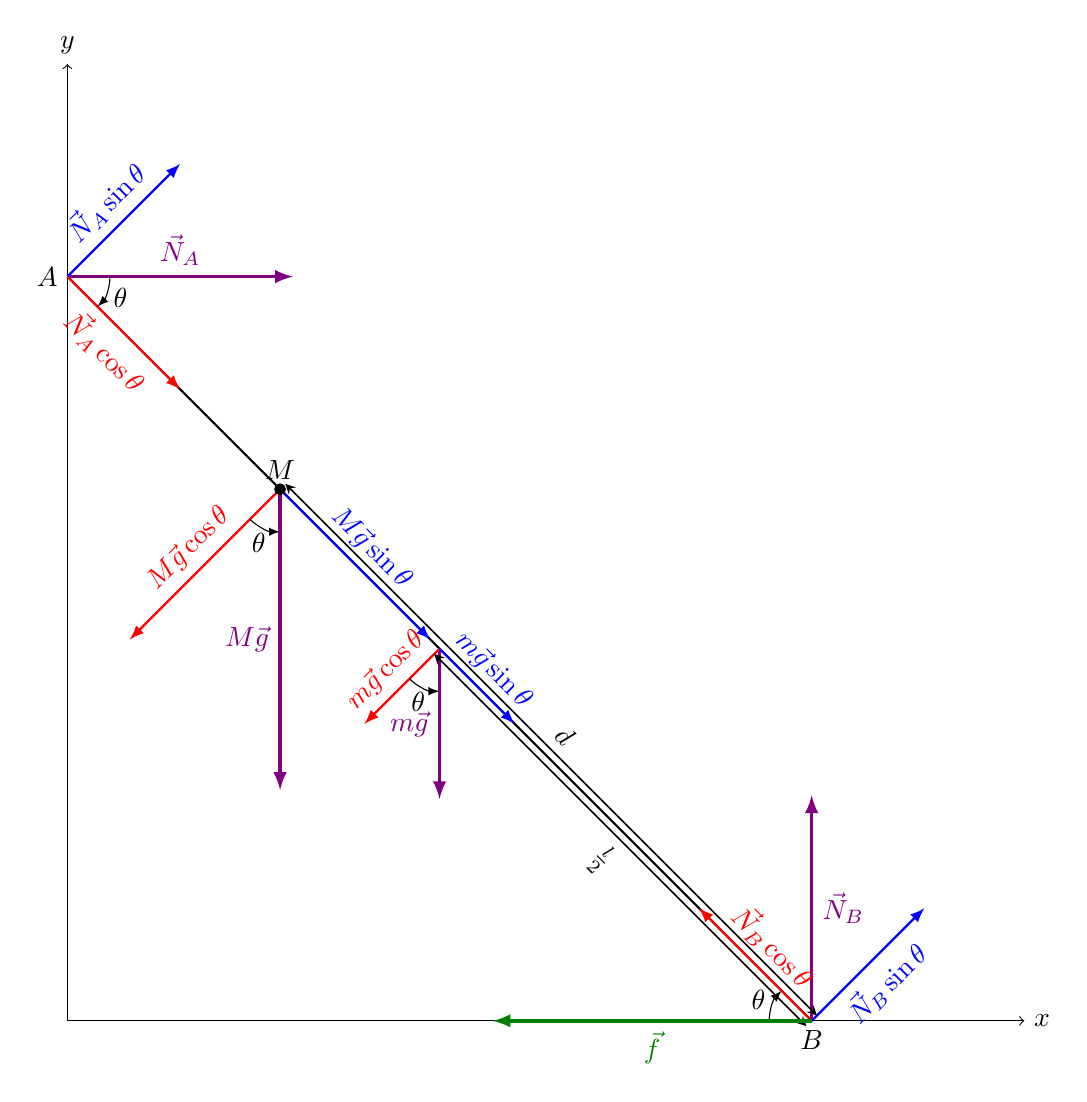
\begin{tikzpicture}[scale=1.35]
	\coordinate [label=right:$x$]		(X)		at	(9,0);
	\coordinate [label=above:$y$]		(Y)		at	(0,9);
	\coordinate							(O)		at	(0,0);
	\coordinate [label=left:$A$]			(A)		at	(0,7);
	\coordinate	[label=below:$B$]		(B)		at	(7,0);
	\coordinate							(C)		at	(3.5,3.5);
	\coordinate	[label=above:$M$]		(M)		at	(2,5);
	
	\draw[<->] (X) -| (Y);
	\draw[thick] (A) -- (B);

	\draw[-latex, very thick, red!50!blue] (A) --++ (0:2.121320343559643) node[midway, above] 	{$\vec{N}_{A}$};
	\draw[-latex, thick, red] (A) --++ (-45:1.5) node[midway, below, sloped] 			{$\vec{N}_{A}\cos\theta$};
	\draw[-latex, thick, blue] (A) --++ (45:1.5) node[midway, above, sloped] 			{$\vec{N}_{A}\sin\theta$};
	\draw[-latex] (A) ++ (0:0.4) arc (0:-45:0.4);
	\node at ($ (A) + (0.5,-0.2)$) {$\theta$};
	
	\draw[-latex, very thick, red!50!blue] (B) --++ (90:2.121320343559643) node[midway, right] 	{$\vec{N}_{B}$};
	\draw[-latex, thick, red] (B) --++ (135:1.5) node[midway, above, sloped] 			{$\vec{N}_{B}\cos\theta$};
	\draw[-latex, thick, blue] (B) --++ (45:1.5) node[midway, below, sloped] 			{$\vec{N}_{B}\sin\theta$};
	\draw[-latex] (B) ++ (180:0.4) arc (180:135:0.4);
	\node at ($ (B) + (-0.5, 0.2)$) {$\theta$};
	
	\draw[-latex, very thick, red!50!blue] (C) --++ (-90:1.414213562373095) node[midway, left] 	{$m\vec{g}$};
	\draw[-latex, thick, red] (C) --++ (-135:1) node[midway, above, sloped] 			{$m\vec{g}\cos\theta$};
	\draw[-latex, thick, blue] (C) --++ (-45:1) node[midway, above, sloped] 			{$m\vec{g}\sin\theta$};
	\draw[-latex] (C) ++ (-135:0.4) arc (-135:-90:0.4);
	\node at ($ (C) + (-0.2, -0.5)$) {$\theta$};
	
	\draw[-latex, very thick, red!50!blue] (M) --++ (-90:2.82842712474619) node[midway, left] 	{$M\vec{g}$};
	\draw[-latex, thick, red] (M) --++ (-135:2) node[midway, above, sloped] 			{$M\vec{g}\cos\theta$};
	\draw[-latex, thick, blue] (M) --++ (-45:2) node[midway, above, sloped] 			{$M\vec{g}\sin\theta$};
	\draw[-latex] (M) ++ (-135:0.4) arc (-135:-90:0.4);
	\node at ($ (M) + (-0.2, -0.5)$) {$\theta$};
	\draw[fill=black] (M) circle(0.5mm);
	
	\draw[<->, >=stealth, line width=0.2mm] ($(B) - (0.5mm,0.5mm)$) -- ($ (C) - (0.5mm,0.5mm)$)
											node[midway, below, sloped] {$\frac{l}{2}$};
	\draw[<->, >=stealth, line width=0.2mm] ($(B) + (0.5mm,0.5mm)$) -- ($ (M) + (0.5mm,0.5mm)$)
											node[midway, above, sloped] {$d$};
											
	\draw[-latex, very thick, green!50!black] (B) --++ (180:3) node[midway, below] 	{$\vec{f}$};
	
\end{tikzpicture}
\end{center}

\paragraph{Solution}
Draw all the forces acting on the ladder : $\vec{N}_A$ (normal force from the wall), $\vec{N}_B$ (normal force from the floor),
$\vec{f}$ (static friction from the floor), $m\vec{}g$ (weight of the ladder) and $M\vec{}g$ (weight of the man).

Note that the ladder is in equilibrium. Thus, we can write
\begin{align*}
	\vec{\tau}_{net}	\;&=\;	0		\\
	\vec{F}_{net,x}		\;&=\;	0		\\
	\vec{F}_{net,y}		\;&=\;	0		\tag{1}
\end{align*}

Also note that when the man is at the maximum height at which the ladder stays in equilibrium, the static friction also attains
its maximum value, i.e.\ , $f = \mu N_B$.\\

Considering the net torque about point $B$, we have
\begin{align*}
	0					\;&=\;	Mgd\cos\theta + \frac{1}{2}mgl - N_A l\sin\theta		\\
	N_A l\sin\theta		\;&=\;	(Mgd + \frac{1}{2}mgl)\cos\theta		\\
	N_A					\;&=\;	\left(\frac{1}{l}Mgd + \frac{1}{2}mg\right)\cot\theta			\tag{2}
\end{align*}

Considering the net force along the $x$-axis, we have
\begin{align*}
	0					\;&=\;	N_A - f								\\
	\mu N_B				\;&=\;	N_A									\tag{3}
\end{align*}

Considering the net force along the $y$-axis, we have
\begin{align*}
	0					\;&=\;	N_B - mg - Mg						\\
	(m + M)g			\;&=\;	\frac{1}{\mu}\left(\frac{1}{l}Mgd + \frac{1}{2}mg\right)\cot\theta	\tag{From (2) and (3)}				\\
	\mu(m + M)g\tan\theta	\;&=\;	\frac{1}{l}Mgd + \frac{1}{2}mg							\\\\
	\Aboxed{d					\;&=\;	\frac{l}{M}\left[\mu(m + M)\tan\theta - \frac{1}{2}m \right]		}		\tag{4}
\end{align*}

\end{document}